\section{Экспериментальное исследование}
\label{sec:5_experiments} \index{5_experiments}

\subsection{Предмет и цели исследования}
\label{subsec:goals}

Предметом исследования являются предложенные подходы к решению задачи: жадный алгоритм с эвристиками EFT и STS; подход на основе ЦЛП. Целями исследования является сравнительный анализ подходов по следующим критериям:

- качество получаемого решения (т.е. значение целевой функции на расписании);

- масштабируемость по времени поиска решения при увеличении размерности входных данных. 

\subsection{Классы графов работ}
\label{subsec:graph_classes}

Используются три класса ориентированных ациклических графов:

\subsubsection{Слоистые графы}
Слоистые графы (рис.~\ref{fig:layered}) характерны для многоэтапных вычислений (цифровая обработка сигналов, научные расчёты).  
Вершины разбиты на последовательные слои, рёбра в основном соединяют вершины соседних слоёв, но допускаются «перескоки» через несколько слоёв.

\begin{figure}[h]
	\centering
	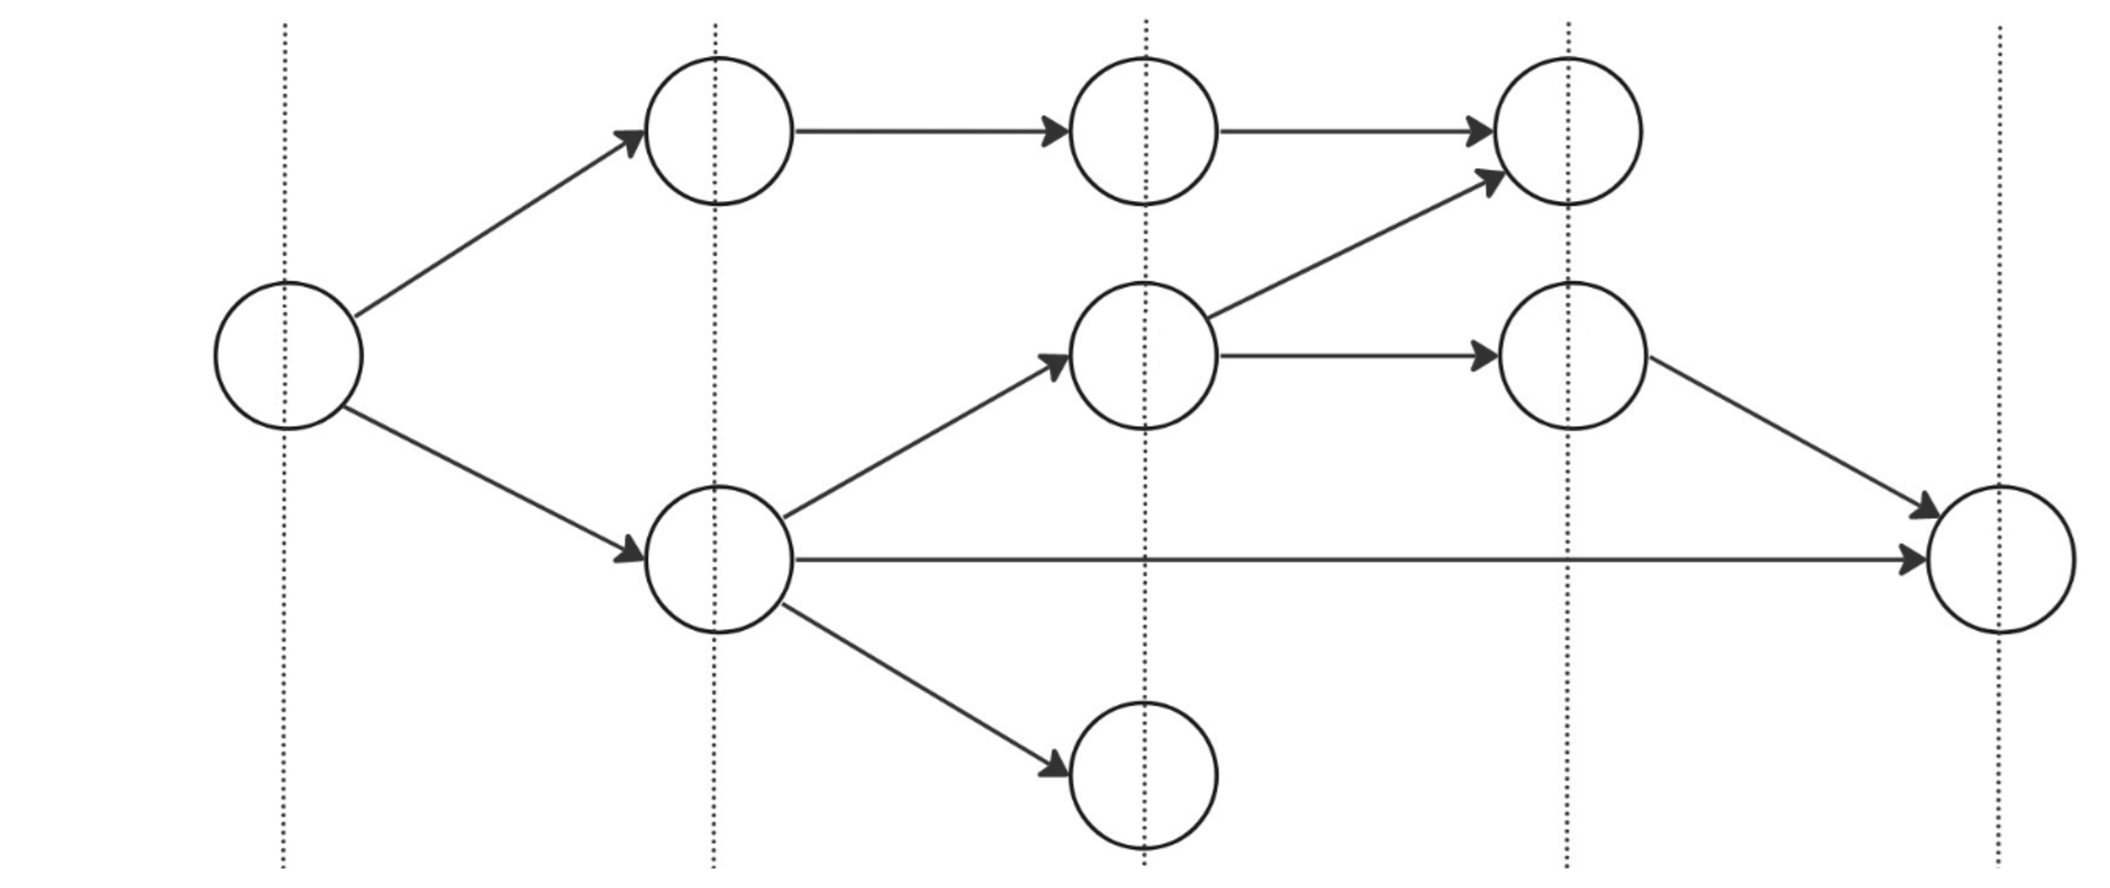
\includegraphics[width=0.5\textwidth]{pictures/layered_graph_scheme.eps}
	\caption{Пример слоистого графа}
	\label{fig:layered}
\end{figure}

\subsubsection{Случайные графы}
Случайные графы (рис.~\ref{fig:random}) генерируются с ограничениями: у каждой вершины не более двух предков и не более шести потомков. Такие графы встречаются, например, при реализации LU- и QR-разложений.

\begin{figure}[h]
	\centering
	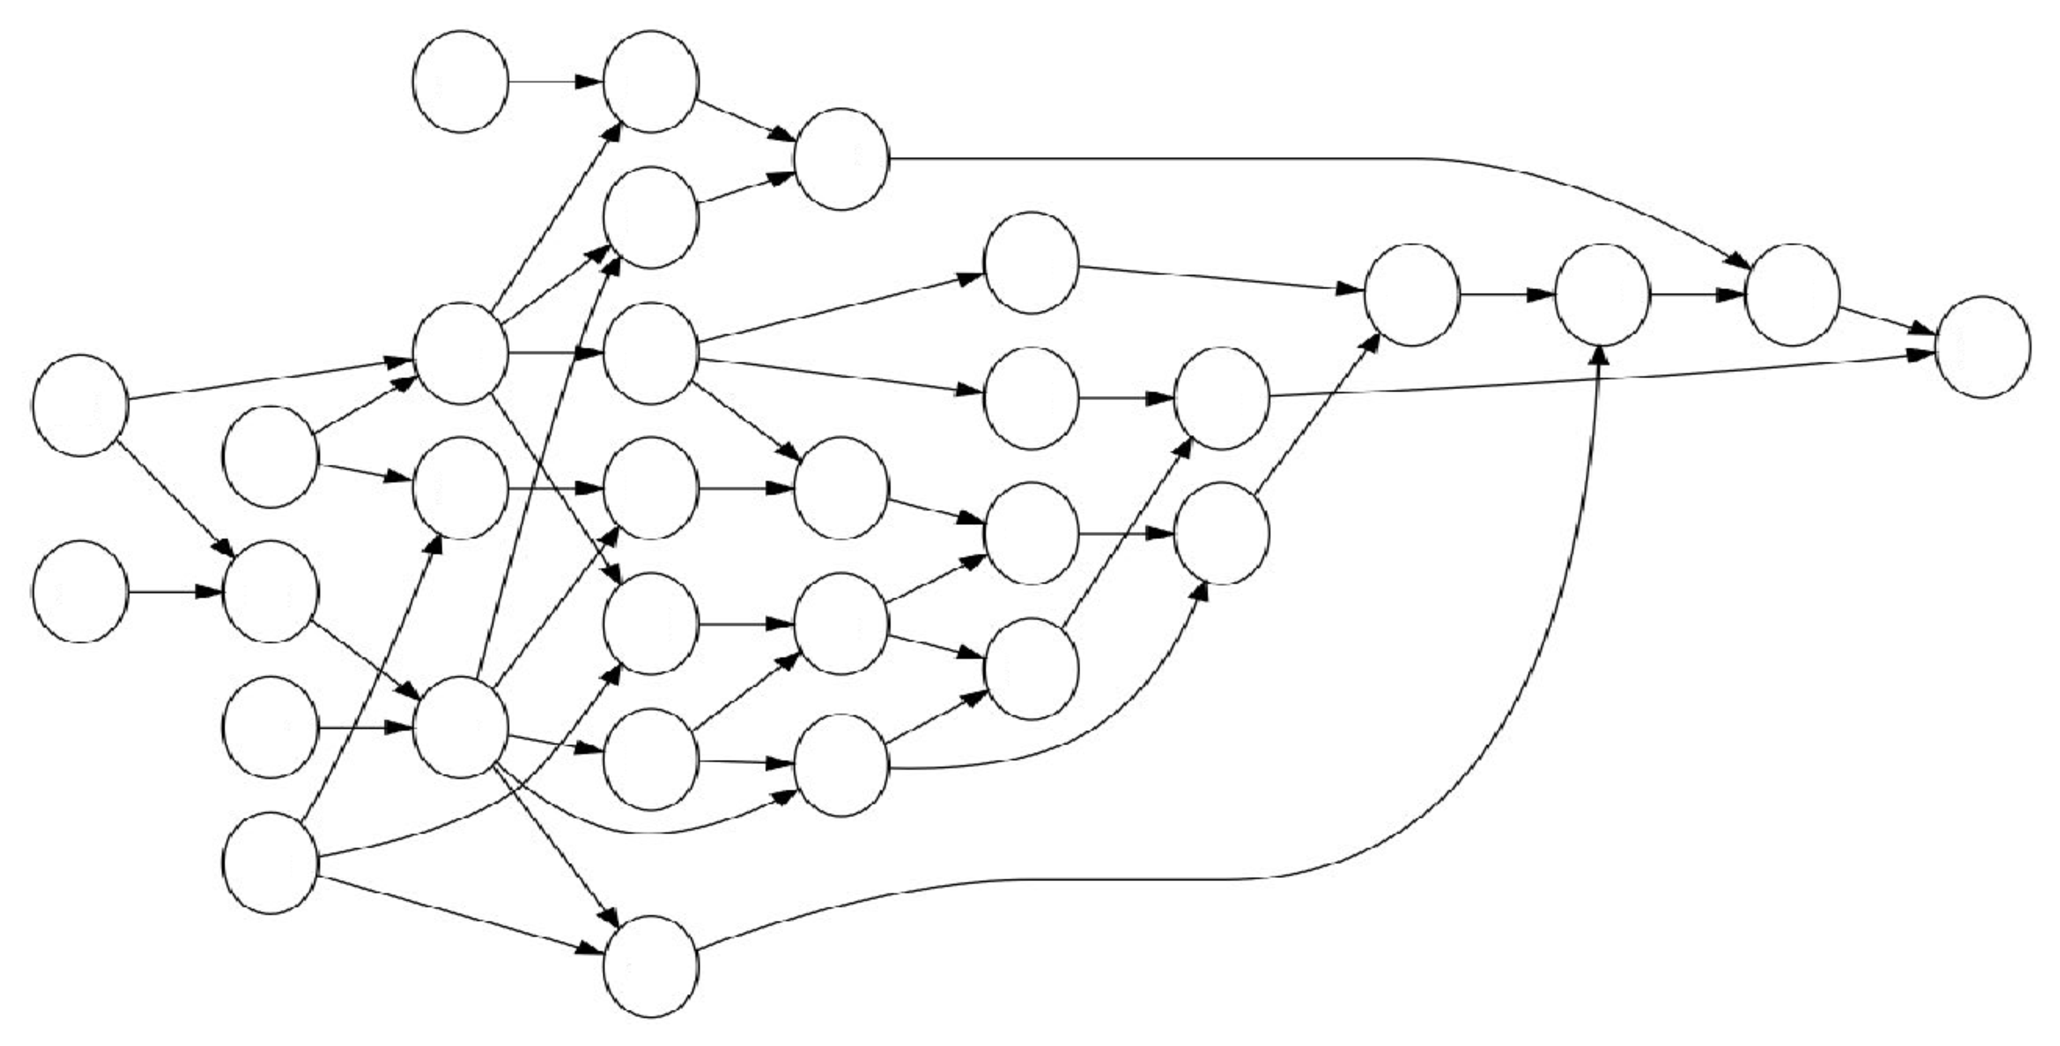
\includegraphics[width=0.5\textwidth]{pictures/random_graph_scheme.eps}
	\caption{Пример случайного графа}
	\label{fig:random}
\end{figure}

\subsubsection{Треугольные графы}
Треугольные графы (рис.~\ref{fig:triangular}) — частный случай слоистых графов, моделирующий метод Гаусса–Жордана.  
Они обладают регулярной структурой: каждый слой содержит на одну вершину меньше предыдущего, рёбра соединяют только соседние слои. Используются только для больших размеров задач.

\begin{figure}[h]
	\centering
	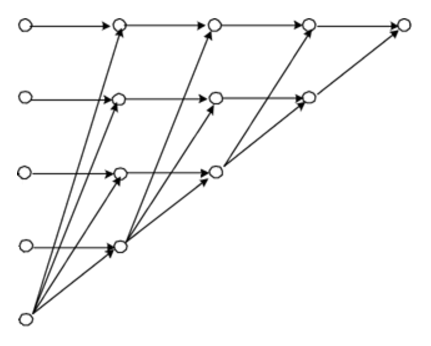
\includegraphics[width=0.5\textwidth]{pictures/triang_graph_scheme.eps}
	\caption{Пример треугольного графа}
	\label{fig:triangular}
\end{figure}

\subsection{Наборы входных данных}
\label{subsec:datasets}

Для каждого из двух исследований (качество и масштабируемость) используются отдельные наборы графов, различающиеся размерностью.  
Все графы имеют следующие общие параметры:

\begin{itemize}
	\item Длительность работы $d_i$ — целое число, равномерно распределённое в диапазоне $[10, 100]$.
	\item Вес каждого буфера — целое число, равномерно распределённое в диапазоне $[1, 100]$.
	\item Для каждой работы используются два варианта формирования буферов:
	\begin{enumerate}
		\item \textbf{Один буфер}: все исходящие рёбра объединены в один буфер указанного веса.
		\item \textbf{Корневое равномерное распределение}: количество буферов равно $\lceil\sqrt{\text{outdeg}}\rceil$, рёбра распределяются по буферам максимально равномерно.
	\end{enumerate}
\end{itemize}

\subsubsection{Малые графы}

\begin{itemize}
	\item \textbf{Слоистые графы}: все размеры $n = 10, 11, \dots, 21$ (по одному графу на размер).
	\item \textbf{Случайные графы}: все размеры $n = 10, 11, \dots, 21$ (по одному графу на размер).
\end{itemize}

\subsubsection{Большие графы}

\begin{itemize}
	\item \textbf{Слоистые графы}: по одному графу для каждого размера $n \in \{55, 210, 496, 990\}$.
	\item \textbf{Случайные графы}: по одному графу для каждого размера $n \in \{55, 210, 496, 990\}$.
	\item \textbf{Треугольные графы}:
	\begin{itemize}
		\item Для оценки качества: по одному графу для каждого размера $n \in \{55, 210, 496, 990\}$
		\item Для оценки масштабируемости: расширенная сетка размеров - по одному графу для каждого размера $n \in \{55, 105, 153, 210, 300, 496, 741, 990\}$ 
	\end{itemize}
\end{itemize}

\subsubsection{Сетка параметров $(P, M)$}

Для каждого графа предварительно определяются:
\begin{itemize}
	\item $P_{\max}$ — максимальное число процессоров, которое может эффективно использовать жадный алгоритм на данном графе при заведомо избыточной памяти.
	\item $M_{\max}$ — максимальная пиковая память, возникающая при выполнении расписания с заведомо избыточным числом процессоров.
\end{itemize}

\noindent \textbf{Число процессоров $P$:}
\begin{itemize}
	\item Если $P_{\max} \ge 50$, то $P \in \{4,\; \lfloor(4+P_{\max})/2\rfloor,\; P_{\max}\}$.
	\item Если $P_{\max} < 50$, то $P \in \{2,\; \lfloor(2+P_{\max})/2\rfloor,\; P_{\max}\}$.
\end{itemize}

\noindent \textbf{Лимит памяти $M$:}
\begin{itemize}
	\item Для малых графов ($n \le 21$): $M_{\min}=1$, поиск ведётся с шагом $1$ до первого допустимого расписания.
	\item Для больших графов ($n \ge 55$): $M_{\min} = \lfloor M_{\max}/10\rfloor$, шаг поиска $\Delta M = \lfloor M_{\max}/100\rfloor$.
	\item В обоих случаях используются три уровня: $M \in \{M_{\min},\; \lfloor(M_{\min}+M_{\max})/2\rfloor,\; M_{\max}\}$.
\end{itemize}

Таким образом, для каждого исходного графа формируется 9 вариантов входных данных ($3\times3$ комбинации $P$ и $M$), на которых проводятся запуски.

\subsection{Результаты экспериментов}

Эксперименты проводились на компьютере со следующими характеристиками:
\begin{itemize}
	\item ЦП: Apple M1
	\item Количество ядер: 8;
	\item Объём ОЗУ: 16 Гбайт;
	\item ОС: macOS Sonoma 14.5.
\end{itemize}

\paragraph{Выбор решателя и схема параллельного запуска}

В качестве решателя задач целочисленного линейного программирования используется SCIP. Выбор обоснован в работе А.К.~Сенюшкиной~\cite{senyushkina2025}, где проведено сравнительное исследование производительности свободно доступных решателей (GLPK, CBC, SCIP) на графах рассматриваемых классов; SCIP показал наилучшие результаты по времени поиска оптимального решения.

Из-за значительной зависимости времени работы решателя от упорядочения переменных и ограничений, а также от добавления транзитивных рёбер (см.~\cite{balashov_senyushkina2024}), применяется метод «параллельного запуска с остановкой по первому успеху». Для каждого входного графа формируются 8 вариантов \texttt{.lp}-файлов, соответствующих комбинациям:
\begin{itemize}
	\item 4 упорядочения вершин и рёбер: \texttt{default}, \texttt{up\_right}, \texttt{down\_left}, \texttt{tiers};
	\item 2 варианта графа: с добавленными транзитивными ограничениями (флаг \texttt{-tr}) и без них.
\end{itemize}
(Упорядочение \texttt{reverse\_tiers} не используется из-за ограниченности числа доступных процессорных ядер.)

Затем скрипт \texttt{run\_scip2.sh} одновременно запускает 8 экземпляров SCIP по одному на каждый вариант. Как только хотя бы один экземпляр завершается с нахождением оптимального решения (статус \texttt{optimal solution found}), все остальные процессы принудительно завершаются. Это позволяет избежать неоправданного ожидания на «медленных» упорядочениях и эффективно использовать доступные вычислительные ресурсы. Лимит времени на каждый экземпляр задаётся в файле \texttt{only\_time.set} (в экспериментах использовалось 3600 секунд).

\subsubsection{Малые графы}

\subsubsection*{Исследование масштабируемости}

\begin{center}
	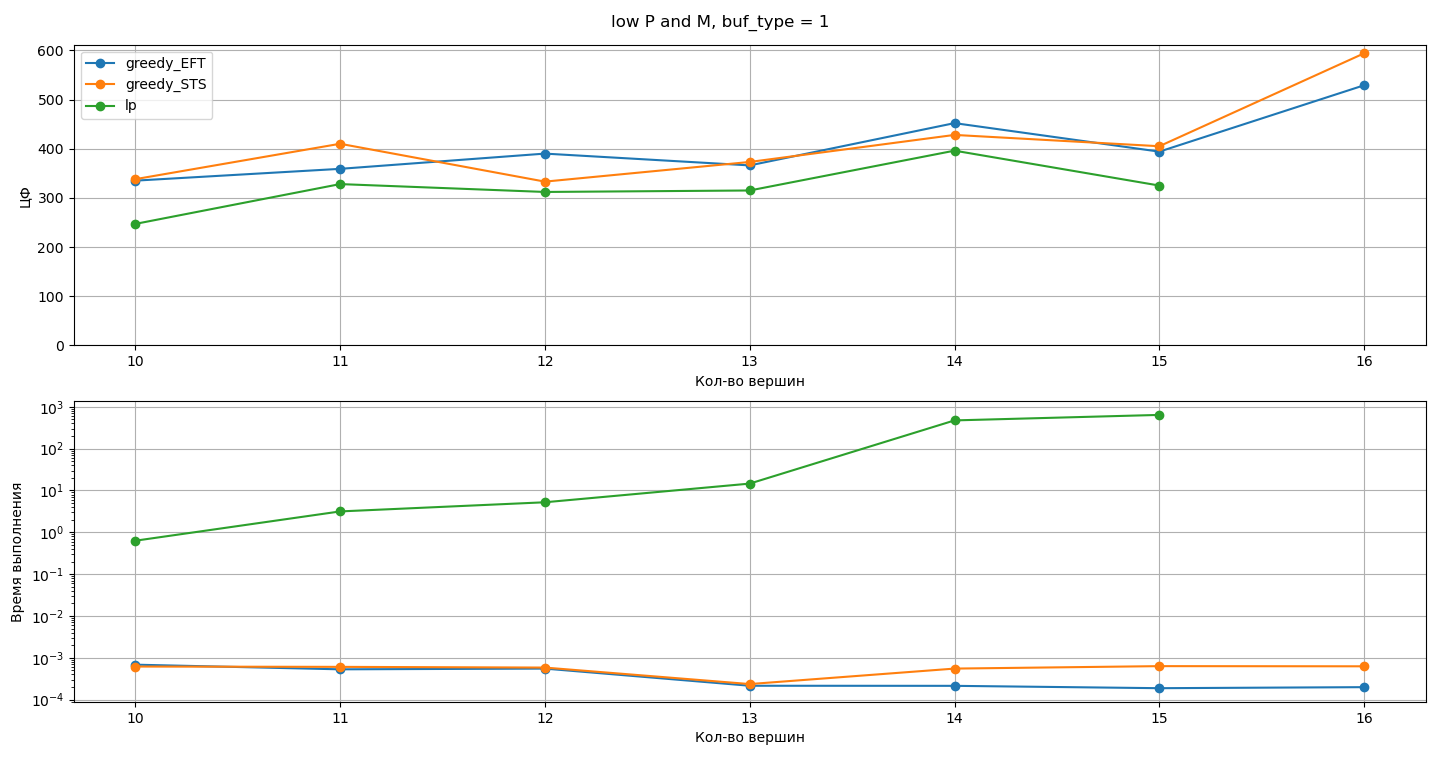
\includegraphics[width=1\textwidth]{pictures/lowPM_1_S.png}
	\captionof{figure}{описание 1}
	\label{fig:scal1}
\end{center}

\begin{center}
	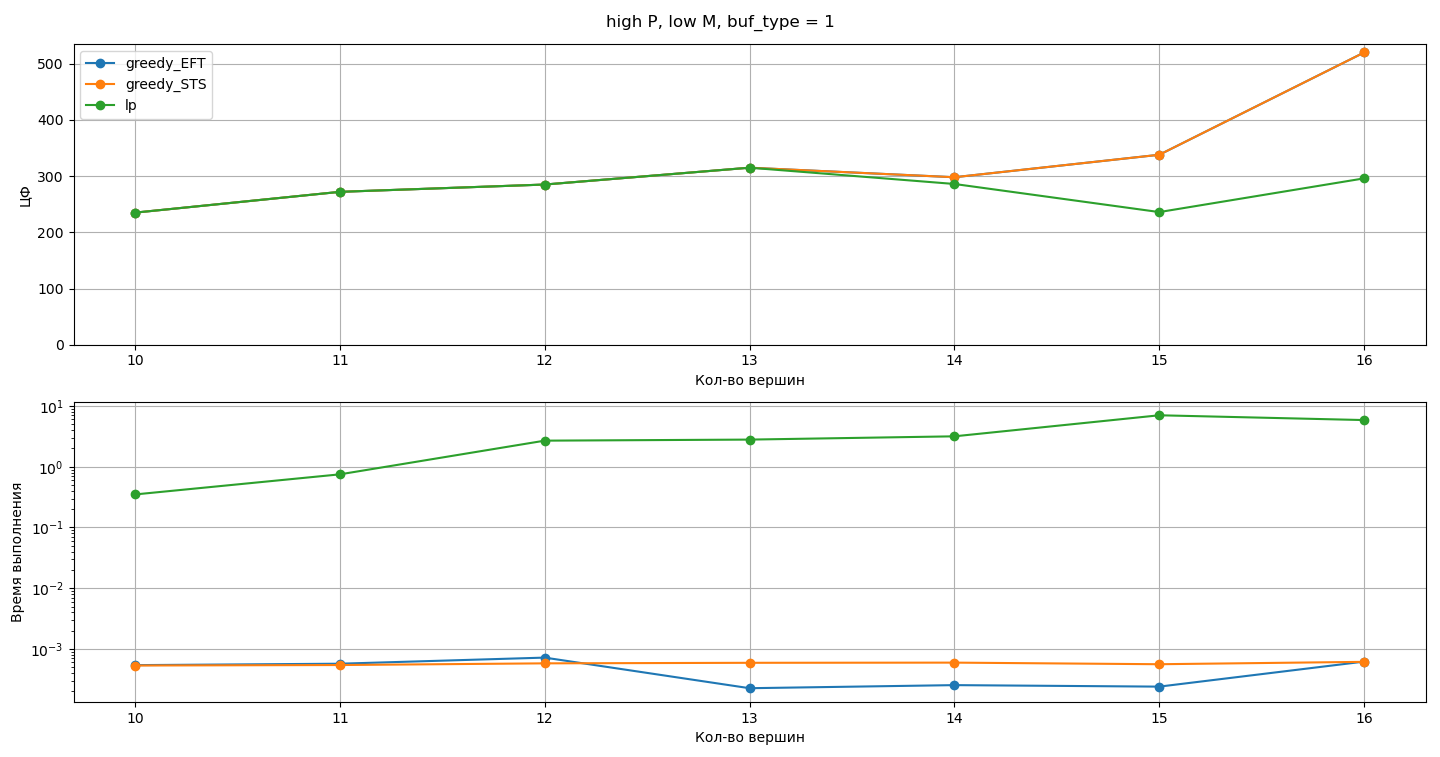
\includegraphics[width=1\textwidth]{pictures/highPlowM_1_S.png}
	\captionof{figure}{описание 2}
	\label{fig:scal2}
\end{center}

\begin{center}
	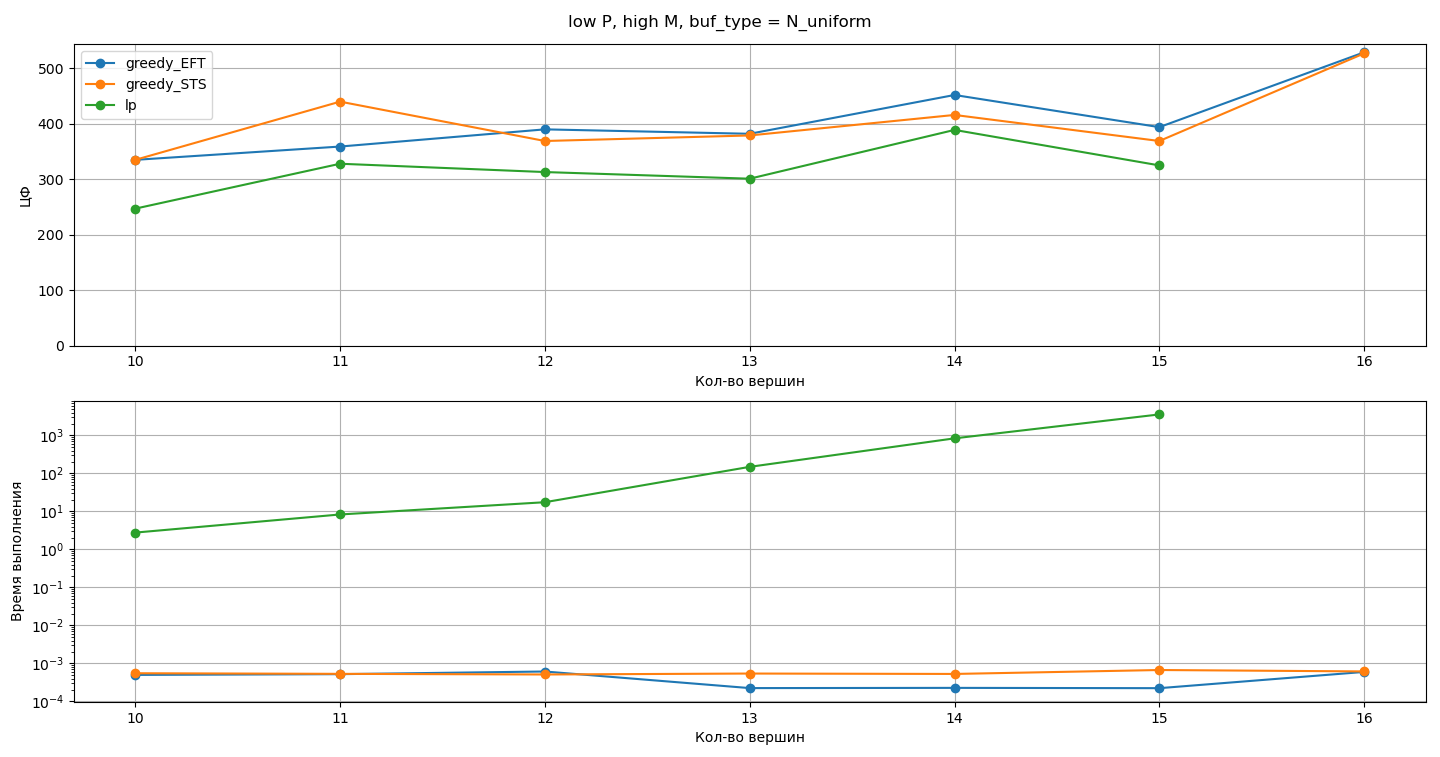
\includegraphics[width=1\textwidth]{pictures/lowPhighM_N_S.png}
	\captionof{figure}{описание 3}
	\label{fig:scal3}
\end{center}

\subsubsection*{Исследование качества решения}

\begin{center}
	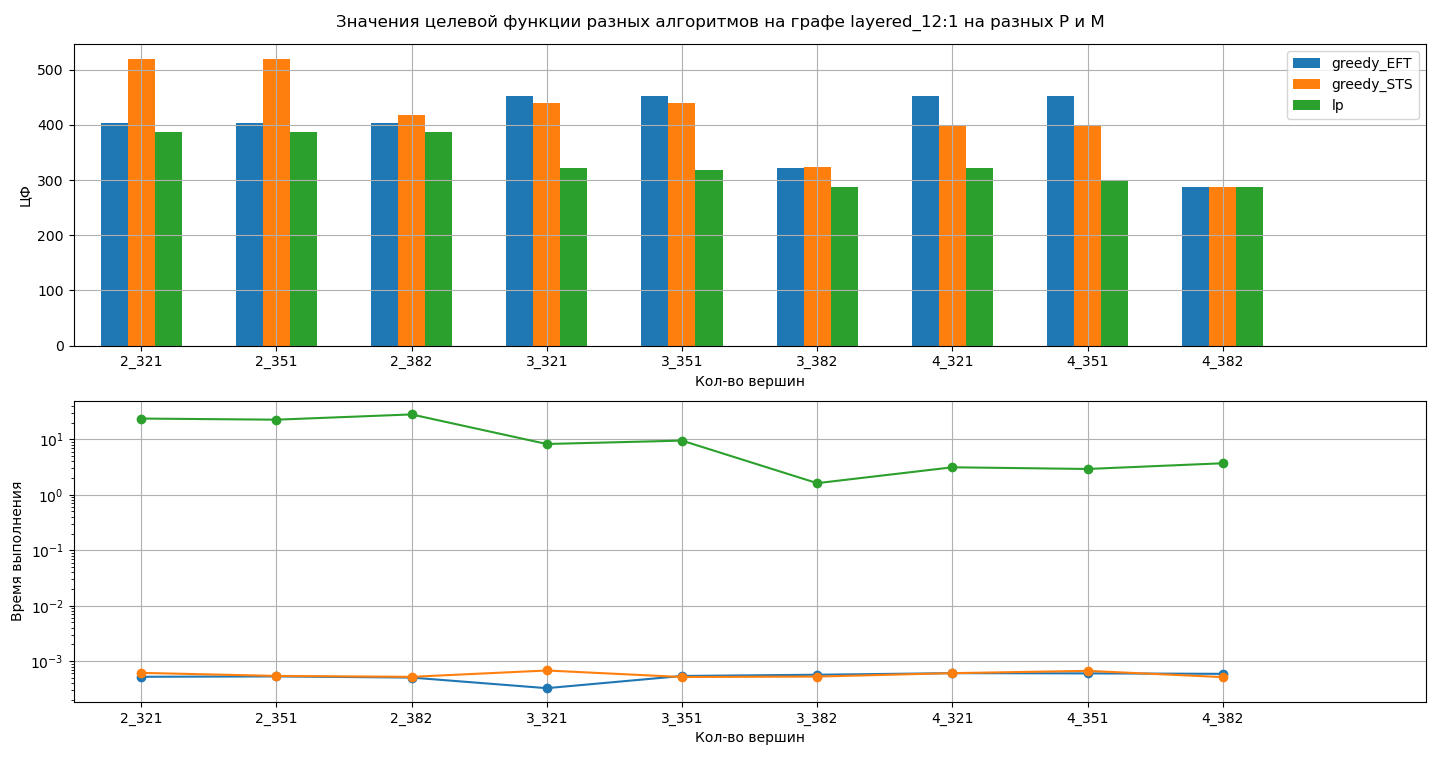
\includegraphics[width=1\textwidth]{pictures/layered_12_1.png}
	\captionof{figure}{описание 4}
	\label{fig:scal3}
\end{center}

\begin{center}
	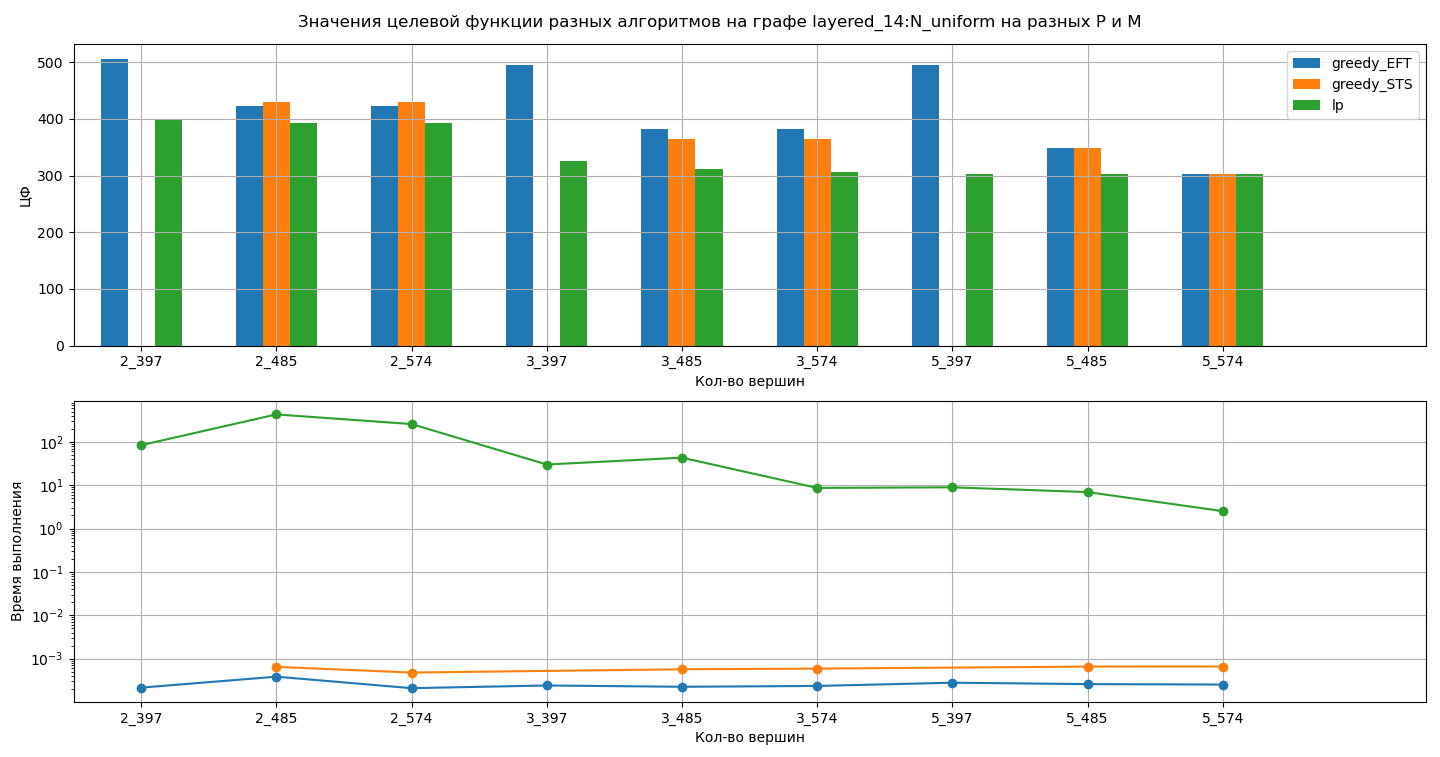
\includegraphics[width=1\textwidth]{pictures/layered_14_N.png}
	\captionof{figure}{описание 5}
	\label{fig:scal3}
\end{center}

\begin{center}
	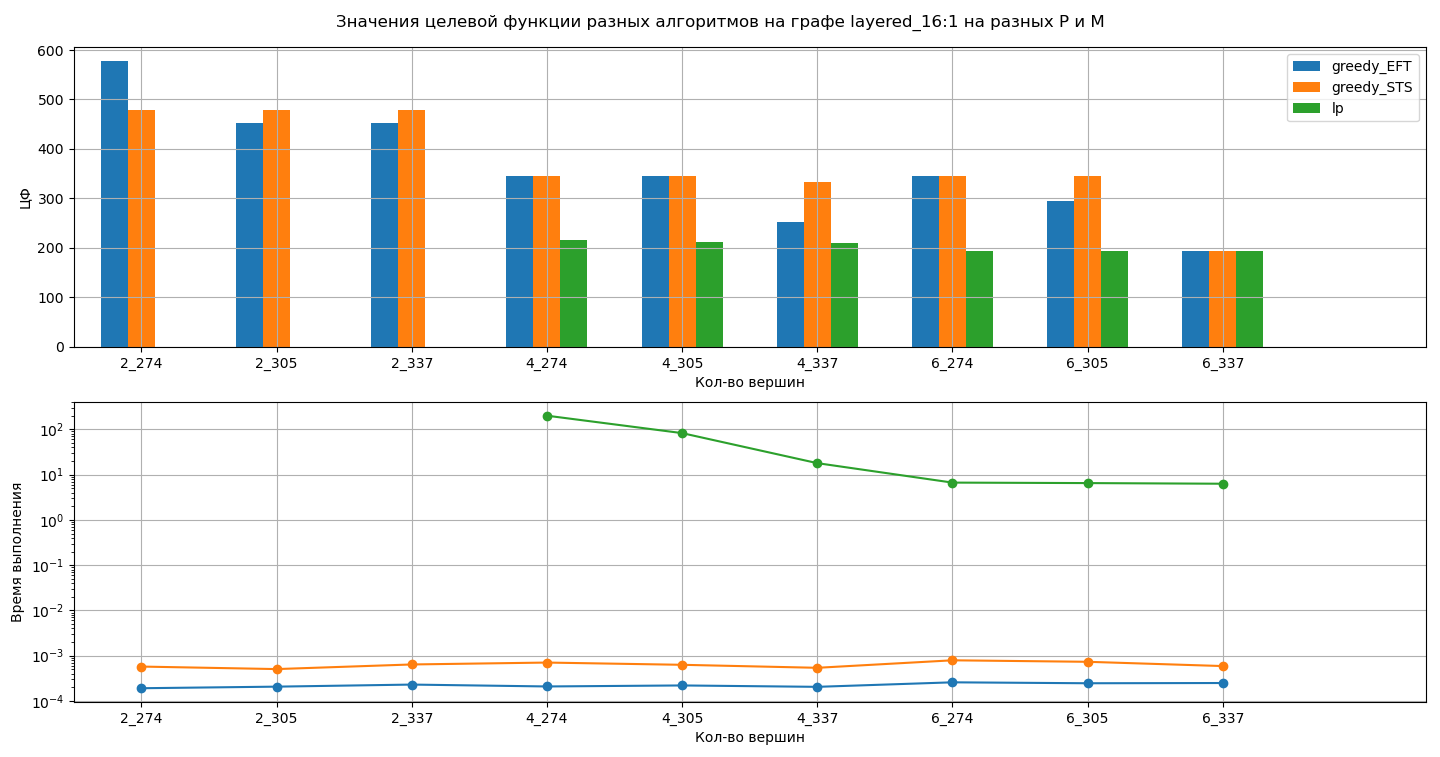
\includegraphics[width=1\textwidth]{pictures/layered_16_1.png}
	\captionof{figure}{описание 6}
	\label{fig:scal3}
\end{center}

\begin{center}
	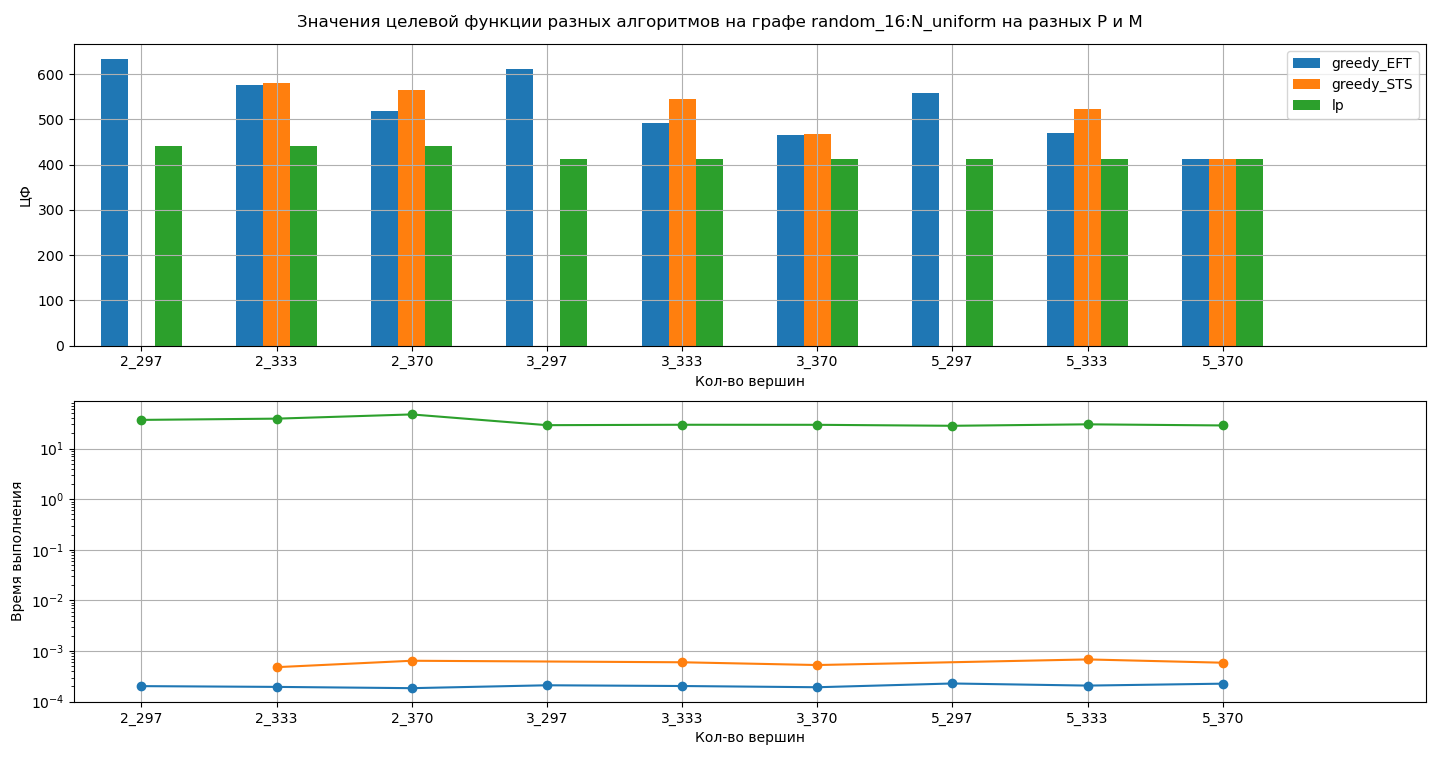
\includegraphics[width=1\textwidth]{pictures/random_16_N.png}
	\captionof{figure}{описание 7}
	\label{fig:scal3}
\end{center}